\documentclass{beamer}
 
\usepackage[utf8]{inputenc}
\usepackage{amsmath}
\usepackage{amssymb}
 
 
%Information to be included in the title page:
\title{C++: A Basic Introduction}
\author{Ben Kettle}
\date{10 Jan 2020}
 
\begin{document}
 
\frame{\titlepage}

\begin{frame}{What is Programming?}

Programming allows us to tell the computer what to do. Instead of relying on software that performs certain functions, we can use programming to make the computer do exactly what we want. 
    
\end{frame}

\begin{frame}{Getting Started}
    \begin{enumerate}
        \item Open CodeBlocks 
\includegraphics[scale=.1]{codeblockslogo.png}
    \end{enumerate}
\end{frame}

\begin{frame}{Create a new File}
    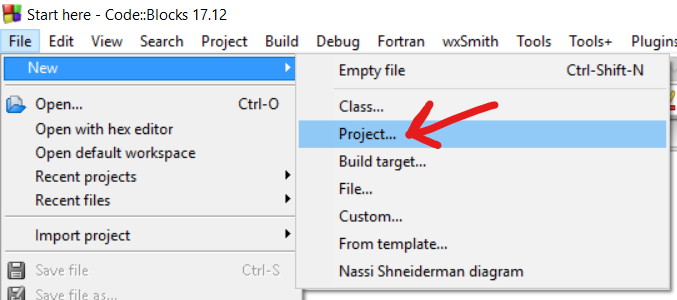
\includegraphics[scale=.5]{codeblockssetup1.png}
\end{frame}

\begin{frame}{Create a New File}
    We want the type to be "Console Application".
    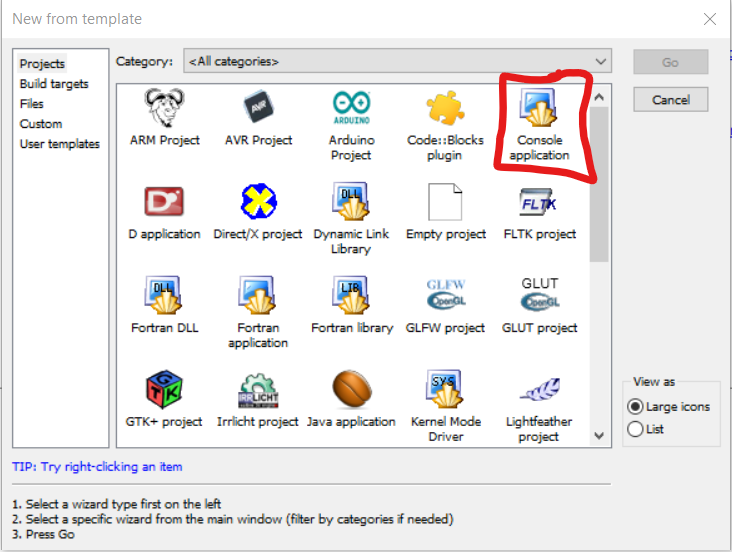
\includegraphics[scale=.5]{codeblockssetup2.png}
\end{frame}

\begin{frame}{Create the file}
     We want to program in C++, so click "C++" then "Next".
     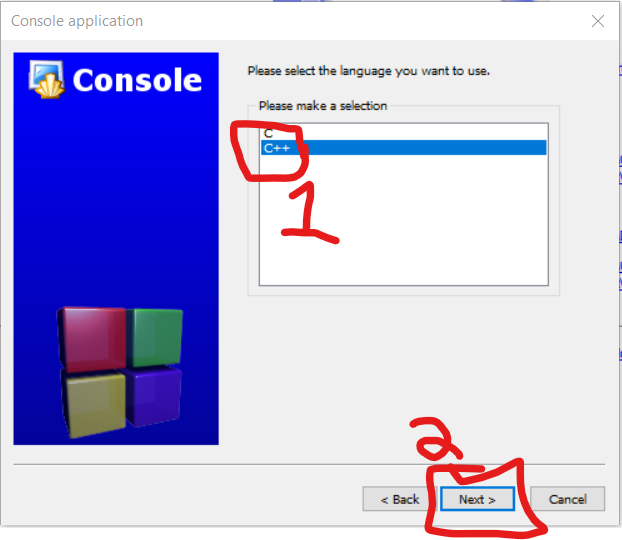
\includegraphics[scale=.6]{codeblockssetup25.png}
    
\end{frame}

\begin{frame}{Name Project}
We now need to choose what to name the project. Type "hello" (or whatever you want) in the "project title" box. Then, click the "..." to select where to put your project.
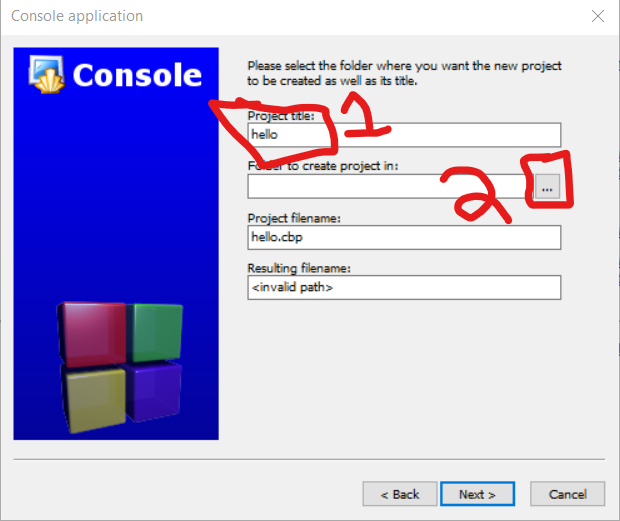
\includegraphics[scale=.5]{codeblockssetup3.png}
    
\end{frame}

\begin{frame}{Place File}
We now need to choose where to store the project files. We'll put them in a folder in My Documents, so click on "Documents" and create a new folder called "cpp_intro". Then, click OK.
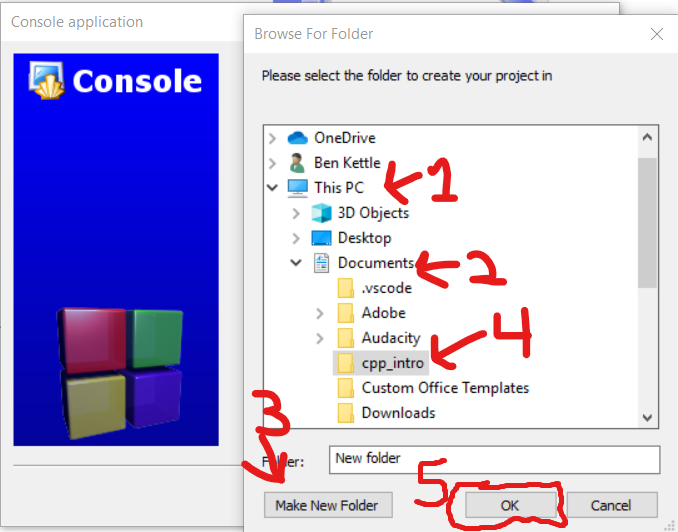
\includegraphics[scale=.45]{codeblockssetup4.png}
    
\end{frame}

\begin{frame}{Open main.cpp}
    Now we are ready to start programming! Expand the "source" section on the left side of the screen and open "main.cpp" by double clicking.
    
    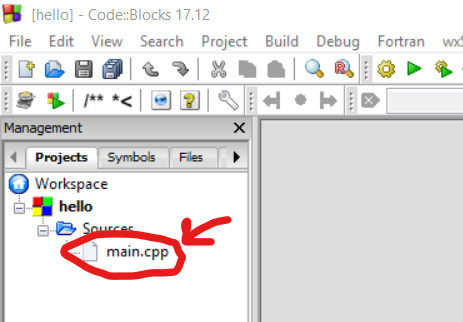
\includegraphics[scale=1]{codeblockssetup5.png}
\end{frame}

\begin{frame}{We have code!}
Your $main.cpp$ file should look like this:
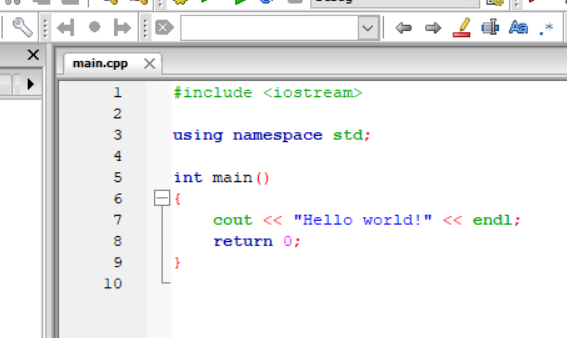
\includegraphics[scale=.7]{codeblockssetup6.png}
We'll have the chance to change this soon, but for now we'll leave it as it is.
    
\end{frame}

\begin{frame}{Build the file}

In order to run our code, we first need to \alert{build} it. This translates your program from code that is easily readable to humans into \alert{assembly} code that the computer can understand. To do this, click "Build" under the "Build" menu.

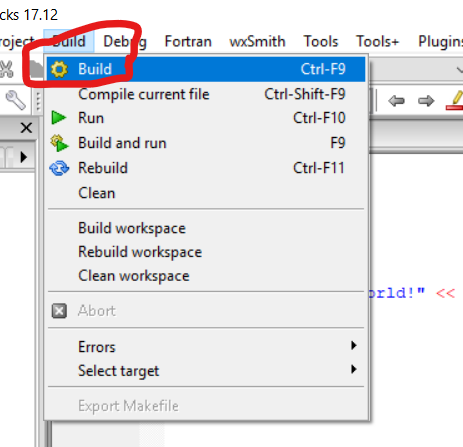
\includegraphics[scale=.6]{codeblockssetup7.png}
    
\end{frame}

\begin{frame}{Run the file}
Once your program finishes building, we can run it! To do this, click "run" under the "build" menu.

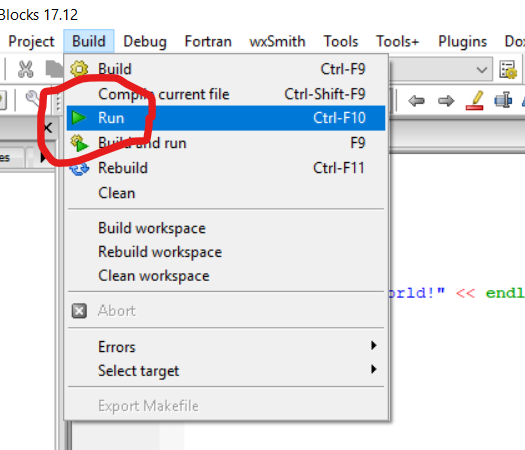
\includegraphics[scale=.6]{codeblockssetup8.png}
    
\end{frame}

\begin{frame}{Your first program!}
Once your program runs, your screen should look like this! This may not look like much, but we'll be able to do much more exciting things soon.

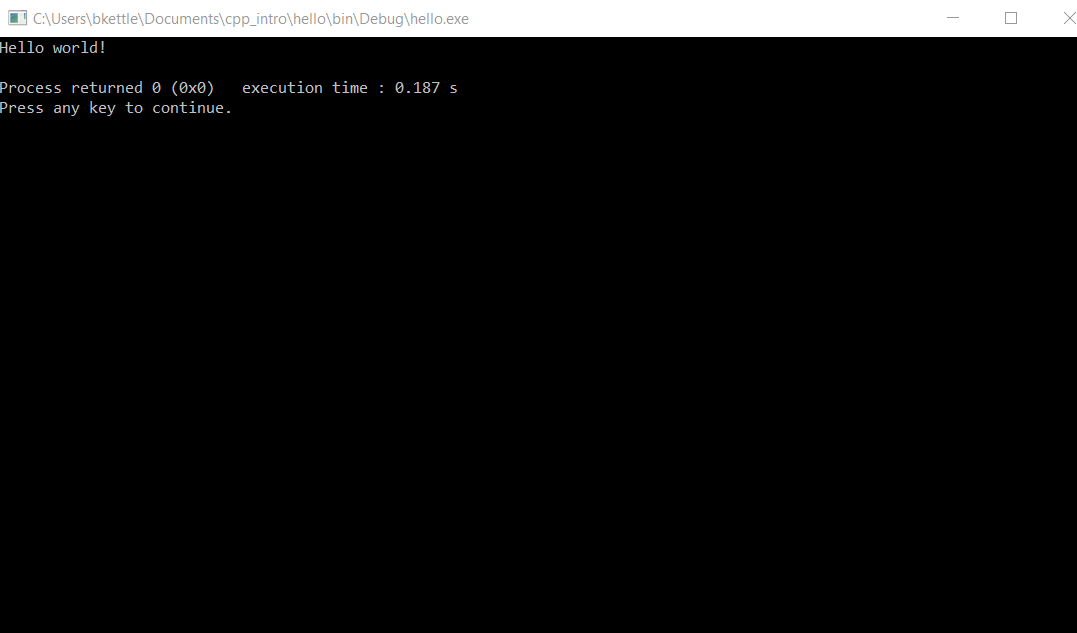
\includegraphics[scale=.4]{codeblockssetup9.png}
    
\end{frame}

\begin{frame}{What's going on here?}
Sure, we made it work, but \textit{why?}

Let's look at the program step by step.
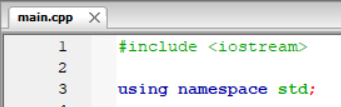
\includegraphics[scale=1]{cpp1.png}

For now, don't worry about these too much. The first line is simply allowing us to get inputs and outputs from the user. The second line is allowing us to use all of the handy functions that C++ comes with.

\end{frame}

\begin{frame}{What's going on here?}

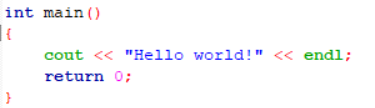
\includegraphics[scale=1]{cpp2.png}

Every C++ application must have a \alert{main()} section. This is the part of code that is run first. The $\{$ and $\}$ symbols define what is inside this section. \newline

The next line is what is doing most of the work here. $cout$ prints to the user, and the $\<\<$ here is writing "Hello world!" to the user. The "endl" is then ending the line, so that the next thing printed will be on the next line. Notice the semicolons at the end of the line: in C++, lines must end with semicolons. You'll learn more about functions soon, but basically this "main()" section has a value attached to it called a "return value". When a function has finished, it sets this value, and that is what the "return 0" line is doing.

\end{frame}

\begin{frame}{Try it!}
    So, we're supposed to make computers do things we want them to, right? Change the text inside the quotation marks to have your program print something else, then Build and Run it as we did before.
\end{frame}

\begin{frame}{Variables}
    Printing is very useful, but doesn't allow us to do much on its own. \alert{Variables} are very important in any programming language, and allow us to store values for later. \newline
    
    For now, delete everything inside the main() section. We're going to create a variable, called $x$. Every variable in C++ must have a \alert{type}. In this case, we want the variable to store numbers---specifically, integers. For this, we use the "int" type. \newline
    On the first line after the $\{$ following main, type "int x;" and hit enter. Here, we're \alert{declaring} a new variable called $x$, and telling the computer that it will be used to store integers. \visible<2->{Now, let's assign a value to the variable. To do this, we use the $=$ sign. On the next line, type "x=4;" and press enter again. We've just stored the number 4 in this variable.} \newline
    \visible<3->{Finally, let's print out the value of that variable! To do this, we'll again write to $cout$. On the line after "x=4;", type \newline "cout $<<$ x $<<$ endl;" and hit enter. Build and run!}

\end{frame}

\begin{frame}{Operations}
    One of the things we'll make the computer do for us most often is math! So let's have it do $4*4=8$. On the line after the print statement we just wrote, type "x=x*4;". This is \alert{reassigning} $x$ to the result of $x*4$. 
    
    \visible<2->{Then, on the following line, copy the line we wrote to print $x$ earlier. 
    
    Q: What do you expect to happen when we run?}
    
    \visible<3->{Try it! Build and run your code as before. Try changing your code to do other operation on other numbers! You can add with $+$, subtract with $-$, and divide with $/$.}
\end{frame}

\begin{frame}{Getting Input}
    It can also be very useful to get input from the user. To do this, we'll do something similar to printing, but in reverse. To try this, we'll make a program that multiplies any number by 4. Remove the line where we assigned "x=4;", and replace it with "cin>>x;".
    
    Build and run this code! If you type a number into the console and press enter, what do you expect it to print? Does it work?
\end{frame}

\begin{frame}{Code so Far}
    At this point, your code should look like this:
    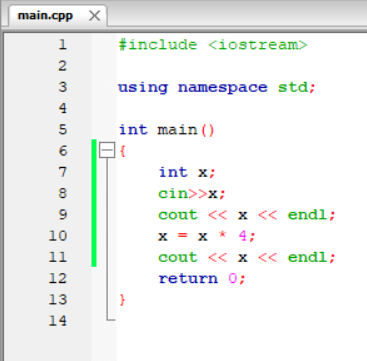
\includegraphics[scale=1]{cpp3.png}
\end{frame}

\begin{frame}{Play around}
    Try combining the things we've done so far to write a cool program.
\end{frame}

\end{document}